% !TEX root = ../thesis.tex
\documentclass[thesis.tex]{subfiles}
\begin{document}



\chapter{Background}
\label{chapter:background}

Tässä osassa selvitetään, mitä tutkimuksen kohteena olevasta aiheesta tiedetään entuudestaan. Selvityksen tulee kattaa tasapainoisesti koko tutkimuskenttä.

\section{Existing solutions}

There is a wide spectrum of technologies available for product authentication. Applications range from the use of inexpensive seals and electronic labels to carefully crafted watermarks and even DNA. These technologies can be categorized in many ways, for example, by their level of security, cost and portability. The focus of this chapter is on commercial smartphone-based product authentication technologies that often trade high precision (or reliability) for better cost-efficiency and portability. The technologies discussed can be considered as competing solutions for the technology developed in this thesis. Due to the nature of the topic the information on most of the technologies is limited in detail. An in-depth overview of product authentication technologies and their background is given in \cite{kuosmanen}.

\begin{figure}[ht]
\centering \includegraphics[width=13.25cm]{images/existing_solutions/smartsure}
\caption{InkSure's SmartSure iPhone application UI. The red rectangle and a virtual spirit level are used to position the smartphone correctly. \cite{inksure} \label{figure:inksure}}
\end{figure}

InkSure's SmartSure technology authenticates products by using a chemical marker (taggant) embedded into a hologram. Upon scanning the hologram, the application verifies it based on the presence of the taggant. The taggant is authenticated via a cloud-based platform that also offers track-and-trace reporting services. The application uses a QR scanner and visual aids to help the user position the smartphone's viewfinder properly over the hologram. \cite{inksure} An image of SmartSure's user interface can be seen in Figure \ref{figure:inksure}.

AlpVision offers a technology called CryptoGlyph\textregistered, which uses a pseudo-random pattern of tiny dots (40-80 microns) printed on the coating of the material to authenticate products. The color and size of the dots are customized based on the packaging color. The authenticity of the product is verified by matching the pattern on the product to one stored in a remote database. As of this writing AlpVision's iOS and Android applications are not publicly available in their respective application stores, but instead distributed as tailored applications ``to meet the client's unique authentication needs''. \cite{alpvision} Figure \ref{figure:alpvision} illustrates how differently sized and color dots affect their visibility and how they are applied to the coating of a material.

\begin{figure}[hb]
\centering \includegraphics[width=\textwidth]{images/existing_solutions/cryptoglyph}
\caption{AlpVision's CryptoGlyph\textregistered{} embeds micro-dots on the coating of a material to create unique invisible patterns for product authentication \cite{alpvision}. \label{figure:alpvision}}
\end{figure}

The ever growing number of NFC-enabled phones (estimated to reach 53\% of the overall market in 2015 according to \cite{frost-sullivan}) has motivated companies to utilize NFC-based technologies for product authentication. Secure and specialized NFC tags have been manufactured by a number of companies since the technology first hit the market in 2006. However, only few companies have developed the software and services around NFC tags in order to provide end-to-end product authentication. A couple of active players in the field are FinnCode\footnote{\url{http://www.finncode.com/}} and Selinko\footnote{\url{http://selinko.com/}}, which both offer a SaaS-based solution for product authentication and manufacture secure NFC tags.

Other notable technologies built around the capabilities of a smartphone include scryptoTRACE\textregistered{} by U-NICA\footnote{\url{http://www.u-nica.com/1320.html}}, CertiEye by Infotoo Ltd.\footnote{\url{http://www.certieye.com/}} and AuthentiGuard by DSS Inc.\footnote{\url{http://www.authentiguard.com/products.html\#tab_authentiguard}}. A summary of the aforementioned technologies is provided in Table \ref{table:existing-solutions}. Next, Chapter \ref{section:photoluminescence} discusses photoluminescence and its applications.

\begin{table}[hb]
	\caption{Existing solutions for smartphone-based product authentication.} \label{table:existing-solutions}

	\begin{center}
	\begin{tabular}{| m{2cm} | m{3.25cm} | m{3cm} | m{3.75cm} |}

		\hline
		\textbf{Company}				&	\textbf{Product name}			&	\textbf{Platforms}			&	\textbf{Technologies} \\ \hline
		InkSure\newline (American)		&	SmartSure						&	iOS						&	- chemical taggant\newline- hologram \\ \hline
		U-NICA\newline (Swiss)			&	scryptoTRACE\textregistered		&	iOS, Android				&	- micro-printing\newline- edge detection \\ \hline
		AlpVision\newline (Swiss)		&	CryptoGlyph\textregistered		&	Customized\footnotesize{*}	&	- micro-printing\newline- pattern recognition \\ \hline
		DSS\newline (American)			&	AuthentiGuard					&	Customized\footnotesize{*}	&	 \\ \hline
		Infotoo\newline (Chinese)		&	CertiEye						&	iOS, Android				&	 \\ \hline
		FinnCode\newline (Finnish)		&									&	iOS, Android				&	- NFC \\ \hline
		Selinko\newline (Belgian)		&									&	Android						&	- NFC \\
		\hline
	\end{tabular}
	\end{center}
	\scriptsize{*} \small{privately distributed, the application is developed according to the client's needs.}
\end{table}

\section{Photoluminescence}
\label{section:photoluminescence}

Photoluminescence, one of the many forms of luminescence (light emission), is a process where a substance absorbs photons (light) and emits back a certain wavelength of light. Photoluminescence can be formally divided into two categories, \emph{fluorescence} and \emph{phosphorescence}, depending on the lifetime of the emission (decay time). Fluorescence typically occurs within a few nanoseconds whereas phosphorescence can last from a few milliseconds to seconds or even hours \cite{luminescence_basics}. Materials that have photoluminescent properties are typically referred to as luminophores (fluorophores and phosphors).

Figure \ref{figure:photoluminescence} illustrates the process of photoluminescence. Photoluminescence is initiated by \emph{photoexcitation}, the absorption of photons causing an electron to move to a higher energy state ($S_0 \rightarrow S_2$). The absorption is followed by internal conversion (IC), where the electron transitions within picoseconds from a higher to a lower energy state. After the electron has reached the lowest excited energy state ($S_1$) it relaxes to the ground state ($S_0$) and emits light (fluorescence), or an intersystem crossing occurs ($S_1 \rightarrow T_1$). The transition from the lowest triplet state to the ground state ($T_1 \rightarrow S_0$) eventually results to the emission of light (phosphorescence).

\begin{figure}[hb]
\centering 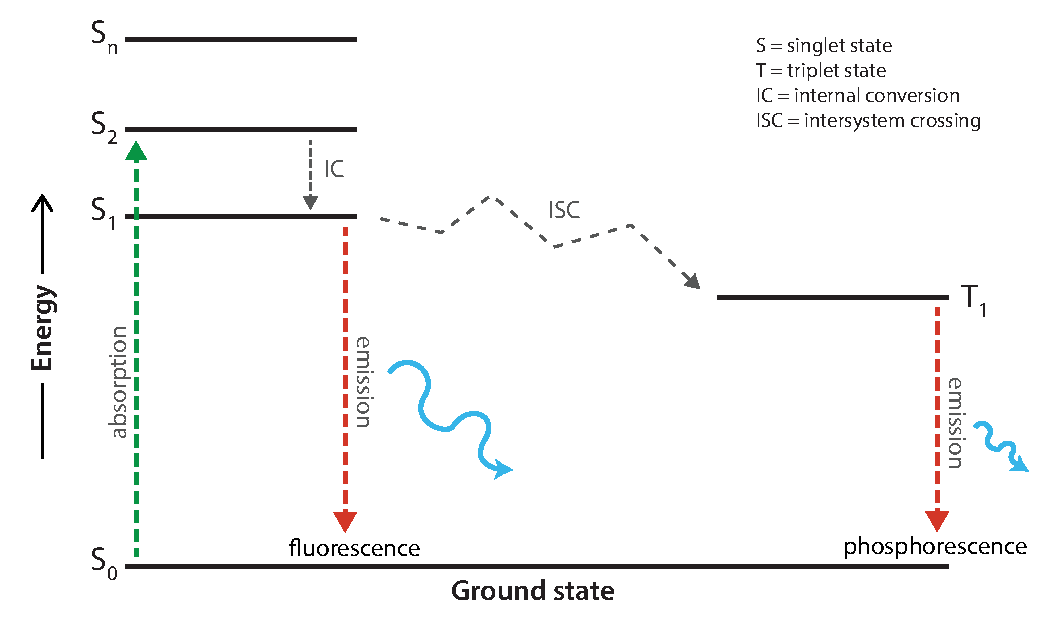
\includegraphics[width=\textwidth]{images/photoluminescence.pdf}
\caption{A simplified Jablonski diagram of photoluminescence. \label{figure:photoluminescence}}
\end{figure}

\noindent Since the energy of the electron at the triplet state is lower than at the singlet state phosphorescence occurs at longer wavelengths of light than fluorescence. Furthermore, the intersystem crossing from the singlet to the triplet state also alters the spin of the electron causing it to decay at a significantly slower pace. Thus, due to the longer excited state lifetime phosphors typically emit light long after the initial absorption of photons. \cite{CEJ}

Luminophores always emit longer wavelengths than they absorb. This is due to the loss of energy within the emission pathway. For example, during IC and ISC transitions some of the excitation energy gets transformed into heat. The difference between the absorption and emission wavelength is known as the Stokes shift. The magnitude of Stokes shift depends on the chemical properties of the luminophore. For fluorophores it is typically in the range of 30-50 nanometers while for phosphors, such as Lanthanide Chelates, it can range up to 200 nanometers. Luminophores are also subject to environmental effects \cite{hemmila}. Changes in temperature, pH, concentration or the amount of dissolved oxygen in the solution affect the intensity of the luminophore and can even shift its emission wavelength \cite{luminescence_basics}.

Photoluminescence can be used for detecting impurities \cite{photoluminescence_use_case_1}, tracing \cite{photoluminescence_use_case_2} and for studying the structure of a system \cite{photoluminescence_use_case_3}. The advantage of luminescence spectroscopy is that it allows analysing materials in a non-destructive and non-invasive manner. Commercially luminescence is used in illuminating watch faces under poor lighting conditions (Figure \ref{figure:photoluminescence_example}). The watch face gets illuminated when its phosphor-coated elements are excited by ionizing radiation. The radiation is induced by a radioactive substance enclosed in the phosphor coating. This form of luminescence is known as radioluminescence. Some less expensive watches use phosphorescence to achieve a similar effect: phosphors exposed to bright light continue glowing in the dark for a short time.

\begin{figure}[hb]
\centering \includegraphics[width=\textwidth]{images/photoluminescence_example}
\caption{Watches use a radioactive substance (typically tritium) to illuminate their elements under poor lighting conditions.\label{figure:photoluminescence_example}}
\end{figure}

When a wavelength of light emitted by a luminophore falls in the visible spectrum of human eye (\mytilde390-700 nm) it creates a perception of a color. Color models are used to encode and represent this information in a medium. Chapter \ref{section:rgbhsv} provides an overview of three commonly used color models and their application areas.

\section{Color models}
\label{section:rgbhsv}

Color models provide an abstract mathematical model for describring colors numerically, typically as a vector of three or four dimensions. A color model alone is only sufficient for relative comparison of colors within that particular model. It is not until the model is given a \textit{context} that it forms a \textit{color space} and the relative colorimetric values get mapped to their absolute counterparts. Here context denotes a set of external (standardized) viewing conditions, in which the colors are expected to be rendered. For example, the standard sRGB color space is based on the RGB color model and assumes an ambient illuminance of 64 lux as per \cite{iec}. The term color model is sometimes referred to as \textit{non-absolute color space} or \textit{relative color space} even if it were less confusing to only speak about color models (relative) and color spaces (absolute).

The next sub-chapters provide a brief overview of a few widely adopted color models: RGB, HSV and YCbCr.

\subsection{RGB}
RGB is the most common color model found in today's computer displays and monitors. It is largely influenced by the historical research on human color vision: the Young–Helmholtz theory of trichromatic color vision, formulized in the 18th century, proposed that color vision is the result of three different photoreceptor cells (cone cells). Later, in 1956 this theory was backed by psychological evidence, which showed that the human retina is particularly sensitive to three groups of wavelengths in the areas of blue, green and red \cite{svaetichin}.

RGB is an \textit{additive} color model meaning that colors are produced by adding together two or more primary colors (red, green or blue). Adding all the primary colors together yields white. All RGB colors are defined relative to the primary colors, as the RGB color model itself does not specify what is meant by red, green and blue colorimetrically. For example, the color of pure yellow would contain all the red and green but no blue: RGB(100\%, 100\%, 0\%). The purpose of color spaces, such as sRGB, is to define the exact values (chromaticities) for the primaries, typically in terms of so called \textit{tristimulus values} (X, Y and Z). The tristimulus values map to a color in the \textit{CIE x-y chromaticity diagram}, which has been established through empirical research to represent all of the chromaticities visible to average human eye \cite{cie}. As seen in Figure \ref{figure:srgb}, a given color space can only produce the colors that fall within its \textit{gamut}, the triangle defined by the chromaticities of its primaries.

\begin{figure}[ht]
\centering \includegraphics[width=10cm]{images/srgb}
\caption{The CIE x-y chromaticity diagram and sRGB gamut (triangle). A color space can only render the subset of colors that are within its gamut.\label{figure:srgb}}
\end{figure}

As evidenced by the wide adoptance of sRGB in digital consumer products, RGB is able to model the human color vision with reasonable accuracy. However, for some use cases there exists better alternatives as covered next in more detail.

\subsection{HSV}

HSV (hue-saturation-value) was developed in the late 1970s originally for computer graphics applications in an attempt to create a more intuitive and perceptually relevant color model. HSV rearranges the cartesian geometry of RGB to a cylindrical coordinate system separating the color information (chroma) from the brightness/intensity information (luma). These geometrical representations of RGB and HSV are depicted in Figure \ref{figure:rgb_hsv}. The ability to decouple luma from chroma brings many benefits in image processing applications. Many basic computer vision algorithms designed for grayscale images, such histogram equalization, canny edge detection or binary thresholding, become trivial in HSV space, since the processing can be done on the luma component (V) alone \cite{color_segmentation}. HSV is also the defacto choice for color pickers as hue, saturation and brightness are both conceptually and perceptually easier to reason about than red, green and blue.

\begin{figure}[ht]
\centering \includegraphics[width=\textwidth]{images/rgb_hsv}
\caption{RGB colors are typically displayed in cartesian coordinates, whereas HSV colors use cylinder coordinates \cite{hsv_cylinder} \cite{rgb_cube}.\label{figure:rgb_hsv}}
\end{figure}

RGB values can be converted into HSV using a simple linear transformation. The formal definition of the transformation can be given as follows:

\begin{align*}
C_{max}&=max(R, G, B),	&	C_{min}&=min(R, G, B),	&	C_{delta}&=C_{max}-C_{min}
\end{align*}
\begin{align*}
V &\leftarrow C_{max}	&
S &\leftarrow
	\begin{cases}
		\frac{C_{delta}}{C_{max}}, & \text{if $V\neq0$}\\
		0, & \text{otherwise}
	\end{cases}			&
H &\leftarrow
	\begin{cases}
		\frac{60(G-B)}{C_{delta}}, & \text{if $V=R$}\vspace{2mm}\\
		\frac{120+60(B-R)}{C_{delta}}, & \text{if $V=G$}\vspace{2mm}\\
		\frac{240+60(R-G)}{C_{delta}}, & \text{if $V=B$}
	\end{cases},
\end{align*}

\noindent where $R, G, B = \{\ x\ \vert\ x \in \mathbb R\ \wedge\ 0 \leq x \leq 1\ \}$.


\subsection{YCbCr}
YCbCr (or YCC) is a family of color spaces used as a part of the color image pipeline of video and digital imaging systems. YCbCr was primarily developed to enable a way of storing and transmitting color information with minimal redundancy, and as such, it can be considered as an intermediate format. Much like HSV it separates luma (Y) from chroma (Cb and Cr) but also compresses the chroma components for improved storage and tranmission capabilities. Because the human visual system is has lower acuity (sensitivity) for color than luminance, the signal can be optimized by compressing the color components \cite{color_vision}. At normal viewing distances this incurs no perceptible loss of quality.

Each YCbCr format uses different subsampling scheme for the compression. The most common YCbCr subsampling (or chroma subsampling) ratios are 4:2:2, 4:1:1 and 4:2:0. The last two digits of the ratio denote how the compressed chrominance information is compressed and encoded as visualized in Figure \ref{figure:ycbcr}. For example, in the 4:2:0 format both the horizontal and vertical resolution of the Cb and Cr chroma components are halved and stored in adjacent columns resulting in a 50\% reduction in required bandwidth. Although different YCbCr schemes offer the same level of compression (e.g. 4:2:0 and 4:1:1) the format should be selected based on which formats the given medium supports to avoid the overhead of conversion.

\begin{figure}[ht]
\centering 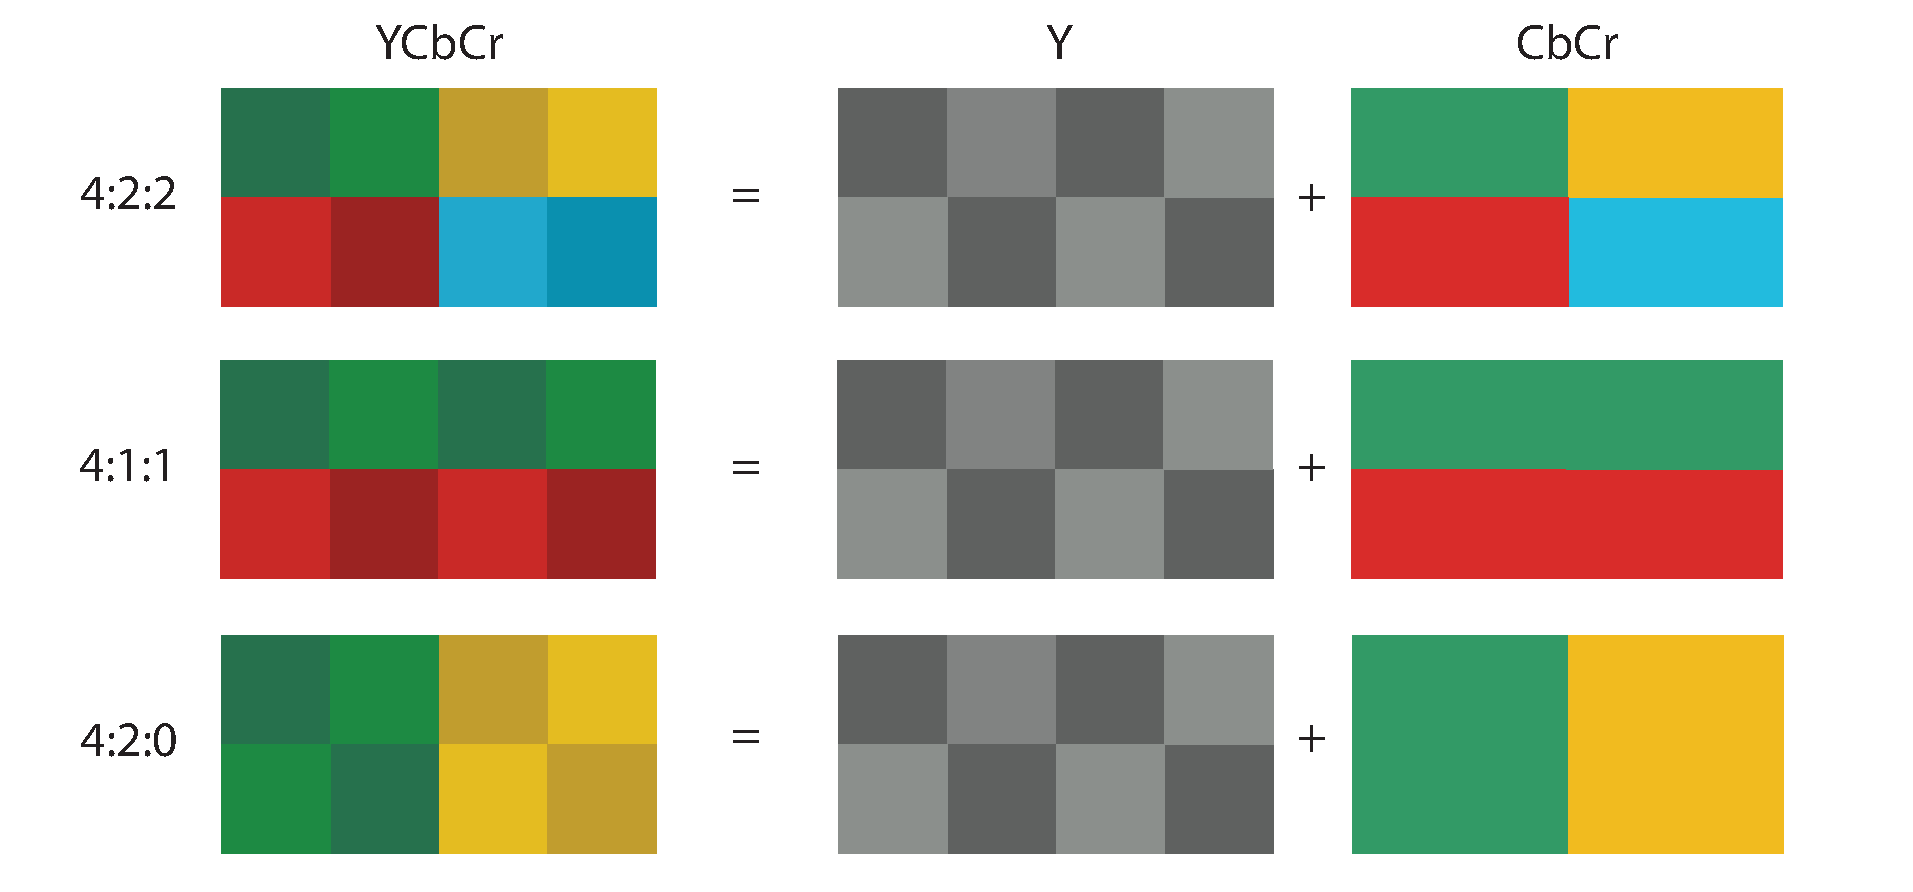
\includegraphics[width=\textwidth]{images/ycbcr}
\caption{YCbCr formats compress and encode chroma in different ways.\label{figure:ycbcr}}
\end{figure}


\section{Mobile Camera Technology}
Since the early 2000s when the first camera phones arrived in the market the technology around mobile cameras has dramatically evolved. The main driving force behind the rapid development has been the competition for customers. Much like with the more traditional point-and-shoot cameras smartphones are marketed largely by their features to attract the mainstream. The increasing number of pixels, better zooming capabilities and features like HDR (High Dynamic Range) photography engage customers but also push the boundaries of mobile camera techonology. And, as smartphones also need to accommodate for other functions, manufacturers are met with further physical (size) and practical (cost and power consumption) constraints. However, these limitations and the competition between smartphone manufacturers foster innovation.

The next chapter will discuss the color image pipeline to help understand the theoretical background behind some of the recent industry innovations introduced briefly in Chapter \ref{chapter:solutions}.

\subsection{Image Pipeline}
Before an image is ready to be rendered or stored in a medium it goes through a series of processing steps commonly referred to as the image pipeline. The image pipeline in modern smartphones is very similar to that of typical DSCs (Digital Still Cameras). However, due to higher price pressure and limitations in available space and power smartphone manufacturers need to compromise. To maximize available space some of the processing is moved from hardware to software, while costs are kept low by using components of lower quality. The exact implementation of the pipeline also varies by manufacturer and the complexity of the smartphone's camera module.

Figure \ref{figure:pipeline} illustrates the different stages of a typical image pipeline. The light reflected by the scene travels through the camera's lens system and an array of filters before hitting the sensor. The pixels (photosites) of the sensor capture the incoming light (photons), which the sensor turns into voltage. The Analog-to-digital converter (ADC) is responsible for converting the voltage into a digital representation. Finally, the signal reaches the ISP (Image Signal Processor), which applies a host of different image processing techniques to form the final image before transmitting it to the medium for display and/or storage.

\begin{figure}[ht]
\centering 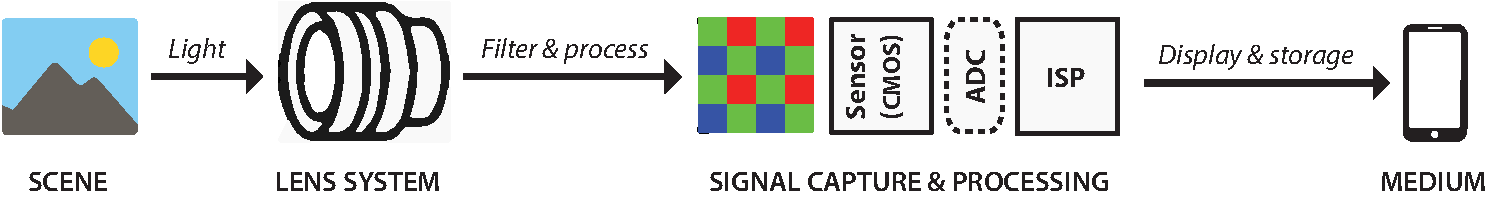
\includegraphics[width=\textwidth]{images/pipeline}
\caption{The different stages of a typical color image pipeline.\label{figure:pipeline}}
\end{figure}

The amount of light falling on the sensor is controlled by the camera's exposure settings. The three factors that affect exposure are the camera's aperture, shutter speed and ISO sensitivity. Aperture defines the effective diameter of the lens opening in terms of a so called \textit{f-number} --- the smaller the f-number the wider the opening. Smartphone cameras typically have a fixed aperture lens with an f-number value between f/2.0 to f/2.4. The reason for using wide fixed apertures is twofold. First, a fixed aperture lens requires less parts and space than a lens of variable aperture, which lowers the costs and complexity of the pipeline. Second, a wide aperture allows for more light to fall on the smartphone's relatively the small sensor. Unlike aperture shutter speed and ISO can often be controlled by the camera software (application). Longer shutter speeds allow more light to be captured whereas a higher ISO increases the sensor's ability to collect photons. However, long shutter speeds are often not suitable for capturing moving objects due to image blur. High ISO values on the other hand affect the quality of the image by introducing noise. Smartphone cameras typically employ an electronic shutter, which is more cost-effective, faster and has less lag than a mechanical shutter. However, the required extra circuitry around the sensor makes the system more prone to noise.

The lens system and the filters laid over the sensor also affect the incoming light. Typically a lens system comprises of multiple stacked lenses, the objective of which are to correct different geometrical and chromatic distortions (abberrations) such as vignette, coma, barrel and pinscushion distortion. Since smartphone camera lenses have both a fixed focal length and aperture the aberrations are easier to account for. After the light has travelled through the lens system and before it reaches the sensor it is anti-aliased, infrared filtered and finally colour sampled using a CFA. \cite{color_pipeline}

\begin{figure}[ht]
\centering 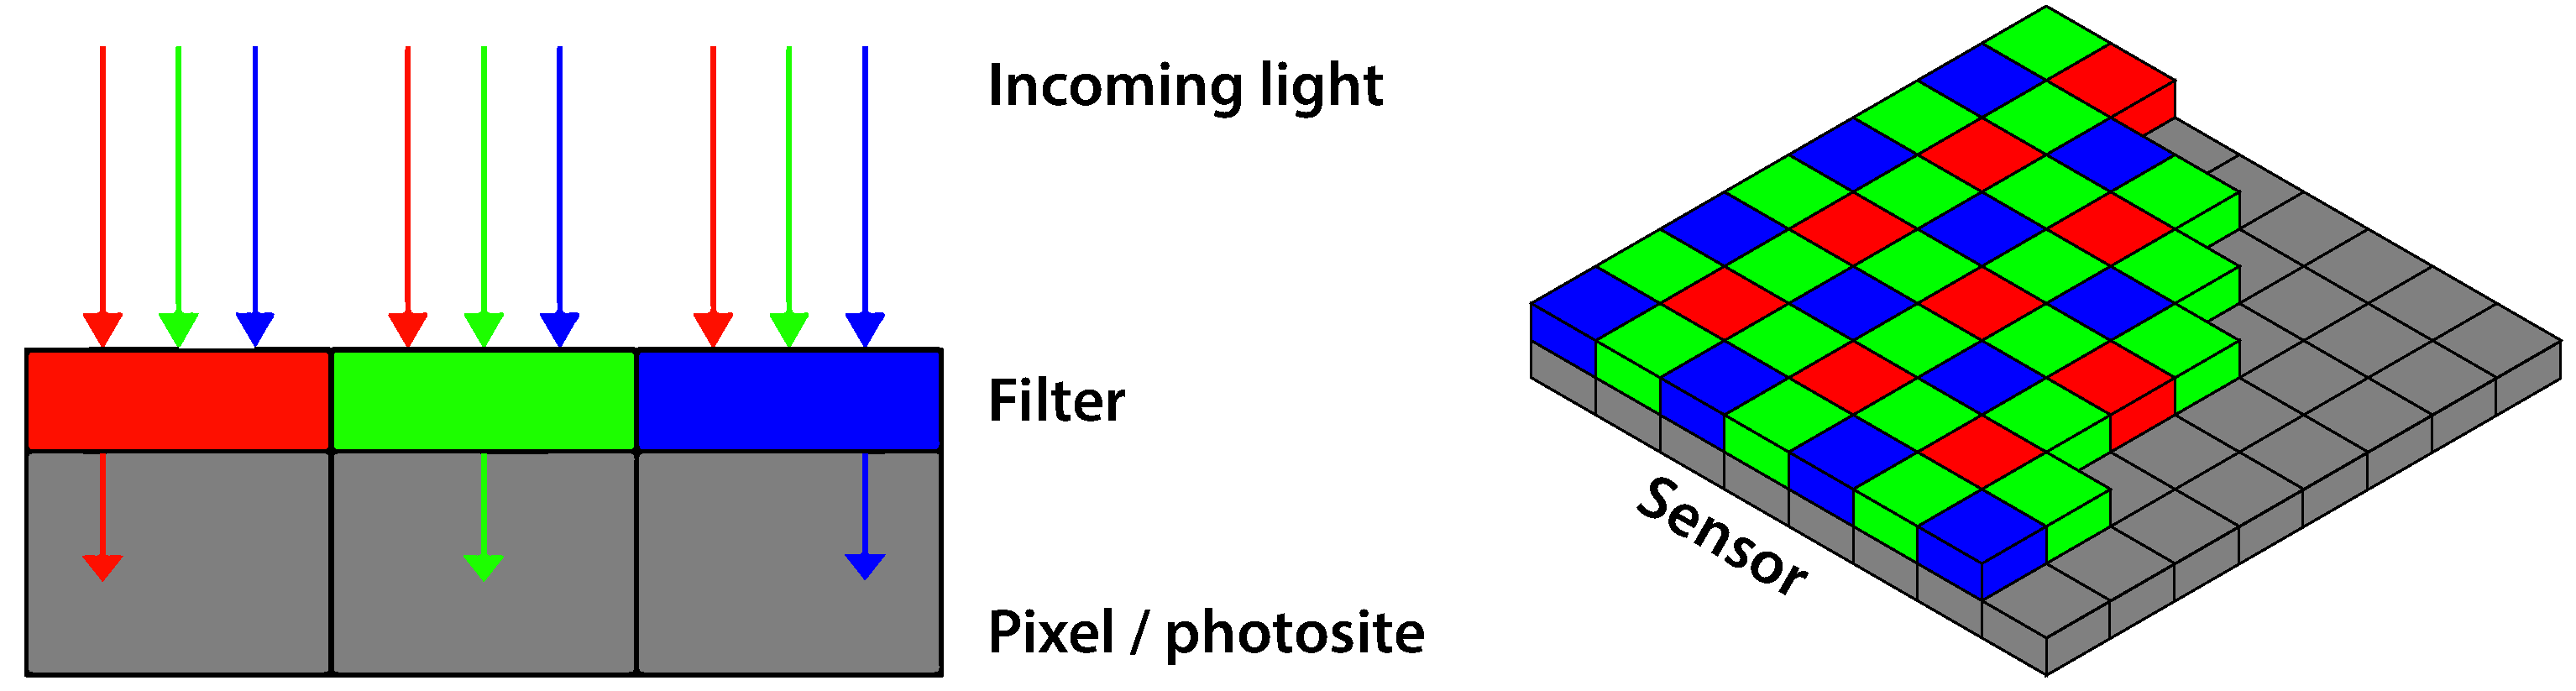
\includegraphics[width=\textwidth]{images/bayer}
\caption{The Bayer filter filters the incident light into intensities of red, green and blue color, which are then interpolated to form the final image. \label{figure:bayer}}
\end{figure}

The purpose of the CFA is to help the sensor distinguish different wavelengths of light since the sensor itself is color blind and only capable of capturing intensities. The sensor is overlaid with the CFA allowing only particular wavelengths of light to be captured by a given pixel. The most common CFA is the \textit{Bayer filter} found in basically every smartphone and consumer level DSC. The Bayer filter consists of alternating rows of red-green and green-blue color filters as illustrated in Figure \ref{figure:bayer}. Due to the fact that the human eye is more sensitive to green light than red or blue the Bayer filter has twice the number of green filters as red or blue. Roughly 2/3 of the incoming light is discarded since each pixel only captures the intensity of one of the three primary colours (wavelengths). Like most commercial DSCs smartphone cameras favour the CMOS sensor technology for its better cost and energy effiency over the more historical CCD technology.

The incomplete colour sampled output of the sensor is reconstructed into a full color image by the ISP. This process is commonly denoted as \textit{demosaicing} or CFA interpolation and it is typically preceded and followed by different image processing techniques such as white balance adjustment, image sharpening and noise reduction. The exact order in which these processes are applied and the type of algorithms used are often company secrets and an active area of competition between manufacturers. In addition to supporting the standard JPEG format some high-end smartphones (e.g. Nokia 1020, Nokia 1520, Nexus 5 and Nexus 6) are able to output unrendered sensor data (RAW). The benefit of RAW format is that it gives the user the ability to apply manual color corrections in a wide-gamut color space before converting the data to a rendered color space (e.g. sRGB) of the output media.

\subsection{Recent Developments}\label{chapter:solutions}

The aim of this chapter is to provide a brief overview of recent developments and emerging solutions in the area of mobile camera technologies. The scope of the discussion is limited to solutions considered relevant in the context of this thesis.

Smartphone cameras are slowly evolving from simple snapshot instruments to devices offering near professional quality image capturing capabilities. The first steps towards this trend were taken during 2012-2013 when Nokia released its first PureView powered phones, Nokia 808 and Nokia 1020. They were the first commercially available smartphones to include sensors bigger than most mid-level compact cameras with a form factor of 1/1.2" and 1/1.5" respectively --- more than twice the size of the typical 1/3" sensor found in most today's smartphones. The Nokia's PureView technology utilizes the camera's large sensor size to provide \textit{lossless zoom} by means of oversampling. For example, the massive 41MP image of the Nokia 1020's can be cropped down to 5MP (A3 size) yielding a magnification factor of 3 without loss in quality. Moreover, cropping the image around its center mitigates aberrations such barrel distortion and vignette. \cite{lumia_1020}

Another relatively new technology featured in the Nokia 1020 was back-illuminated sensor (BI). After the first BI powered smartphones appeared in the market in 2010 (HTC Evo 4G) and 2011 (Apple iPhone 4) the technology has seen wide adoptance, especially in high-end smartphones. BI is a technology targeted for improving the sensitivity of CMOS sensors. While the more traditional front-illuminated CMOS sensors are less expensive and easier to manufacture, BI achieves better sensitivity by novel arrangement of imaging elements and circuitry underneath the sensor surface.

The innovations behind Nokia's flagship phones and others alike have mainly focused on optimizing existing hardware. Sony however has taken a different approach with its QX product line first released in late 2013. Sony's QX products include different \textit{smartphone attachable lens-style cameras}, which are mountable camera modules that can used to replace the smartphone's built-in camera (Figure \ref{figure:sony-qx}). The idea is similar to that of professional DSLRs, which allow different lenses to be mounted on the camera body. While the Sony QX camera modules have internal storage capabilities they require a Wi-Fi connection for communicating with and transferring data to the smartphone.

\begin{figure}[ht]
\centering \includegraphics[width=\textwidth]{images/sony_qx.jpg}
\caption{Sony's interchangeable camera modules: QX10 lens camera (left) and QX30 lens mount (middle) featuring a APS-C sized sensor.\label{figure:sony-qx}}
\end{figure}

In the near future Google's Project Ara aims to take \textit{smartphone modularization} a step further. The goal of the project is to offer a base smartphone model that can be customized and extended by interchangeable third-party components. For example, in low-light conditions less noisy images could be produced by mounting a camera module having bigger pixels or wider aperture. The modular approach of Ara could potentially allow easy integration of specialized components like NVIDIA Chimera\texttrademark\ to make smartphones a suitable platform for different computational photography applications.

Smartphone modularity has also been in Apple's radar as evidenced by patents \cite{apple_patent_camera_module_3}\cite{apple_patent_camera_module_4}\cite{apple_patent_camera_module_5} acquired for interchangeable iPhone camera lenses. Other innovations Apple is working on include multi-sensor camera and refocusable imaging mode \cite{apple_patent_camera_module_1}\cite{apple_patent_camera_module_2}. The multi-sensor system uses three separate sensors, one for luminance and two for chrominance, to produce images with both higher resolution and color accuracy. The raw data from the three sensors is read by the ISP to form a composite color picture. Apple's patent for the refocusable camera describes a plenoptic camera (light-field camera) with a movable microlens array. Plenoptic cameras use a microlens array situated between the sensor and the lens system to capture the intensity of light as a function of position and angle. The ISP can use this information in the post processing phase to refocus the image or to obtain depth information of the scene. The spatial resolution of the image is however constrained by the number of lenses in the microlens array since one microlens can accurately sample light only for one spatial point (pixel). Several so called \textit{super-resolution} techniques have been proposed to overcome this limitation \cite{plenoptic_1}\cite{plenoptic_2}\cite{plenoptic_3}.

\begin{figure}[ht]
\centering \includegraphics[width=\textwidth]{images/htc-ufocus.jpg}
\caption{HTC One M8 is capable of depth based image segmentation, which its UFocus\texttrademark\ technology uses for creating a fake artistic bokeh effect.\label{figure:htc-ufocus}}
\end{figure}

In early 2014 HTC released HTC One M8 featuring a dual camera system (Duo Camera). The two cameras have a fixed offset, which allows the Duo Camera to capture the visual disparity of an object. The ISP can use this information to obtain depth information --- the larger the disparity of an object the further away it is from the focal plane (sensor). The more accurate estimation of an object's distance allows the Duo Camera to provide faster auto-focus (AF) compared to the typical single-camera systems that often use a contrast detection based approach. Figure \ref{figure:htc-ufocus} provides an example of HTC One M8's UFocus\texttrademark\ technology, which uses the depth capturing capability of the Duo Camera to create a fake bokeh effect.

Advancements in mobile camera technology have not only taken place in hardware but in software as well. In 2014 Apple, Android and Microsoft released new versions of their operating systems (iOS 8, Android 5.0 Lollipop and Windows Phone 8.1 respectively) all featuring, for the first time, APIs for manual camera control. As features like manual control, RAW shooting and OIS are becoming increasingly common in smartphones it is evident that the technological gap between mobile cameras and high-end DSCs is shrinking. Convergence of media and the innovations it introduces will help push these technological boundaries further.

\section{Hybrid Mobile Landscape}

Mobile applications can be generally developed as native, hybrid or web applications. A native implementation offers the highest perfomance (least overhead) and the widest access to device APIs (sensors, storage, contacts). However, building a mobile web application allows better portability and code re-use across platforms and devices, which reduces development time and costs. Hybrid mobile applications (or, hybrid apps) combine the best of both worlds by leveraging web technologies to deploy native-like mobile applications to a broad range of smartphones. Hybrid apps can be further divided into \textit{WebView apps} and \textit{Compiled Hybrid apps}. WebView apps use web technologies (HTML, CSS and JavaScript) and the platform's native browser component (commonly known as the web view) to communicate with the platform's native layer. Compiled Hybrid apps on the other hand allow code written in one programming language to target multiple platforms by compiling it to platform-specific native code. The following will focus on WebView apps with a brief overview on different Compiled Hybrid app solutions towards the end of the chapter.

A widely popular tool for building \textit{WebView apps} is Apache Cordova, an open-source cross-platform mobile development framework originally known as PhoneGap and developed by Nitobi. After Adobe's acquisition of Nitobi in 2011 the PhoneGap codebase was contributed to the Apache Software Foundation to start the Apache Cordova project. Nowadays Adobe PhoneGap exists as a distribution of Apache Cordova including additional services such as Adobe PhoneGap Build and Adobe PhoneGap Enterprise. Since the release of Cordova in 2012 numerous commercial \textit{hybrid mobile development platforms} have emerged alongside Adobe's PhoneGap product line. Most notabe of these include products such as Telerik Platform, Ionic Platform, AppGyver Steroids, Sencha Touch, Trigger.io, Appery.io, Monaca and Intel XDK. They provide additional tooling (CLI programs, IDE plugins), generic UI components and SaaS/BaaS solutions (storage, analytics, notifications) to both streamline and address the challenges of developing and deploying hybrid mobile applications for various platforms.

Unlike its commercial counterparts Cordova does not provide any readily available UI components or a client-side MVC framework. To meet this need several UI frameworks optimized for hybrid mobile applications have been developed. These frameworks minimize development overhead by addressing common platform-specific quirks and by providing platform-specific styles and performance optimizations (e.g. removing the 300ms click delay designed for desktop browsers \cite{click_delay}). The most popular of these cross-platform mobile UI frameworks, the JavaScript libraries they depend on and platforms they support are listed in Table \ref{table:cross-platform-mobile-ui-frameworks}.

\begin{table}[ht]
	\caption{Popular cross-platform mobile UI frameworks.} \label{table:cross-platform-mobile-ui-frameworks}

	\begin{center}
	\begin{tabular}{| m{3.5cm} | m{3.5cm} | m{4.75cm} |}

		\hline
		\textbf{Framework}	&	\textbf{Dependencies}		&	\textbf{Supported platforms}		\\ \hline

		Ionic				&	AngularJS					&	iOS, Android						\\ \hline
		Kendo UI			&	jQuery						&	iOS, Android, WP8					\\ \hline
		Onsen UI			&	AngularJS					&	iOS, Android						\\ \hline
		Reapp				&	React						&	iOS 								\\ \hline
		ChocolateChipUI 	&	jQuery \footnotesize{*}		&	iOS, Android, WP8					\\ \hline
		jQuery Mobile 		&	jQuery						&	iOS, Android, WP8 \footnotesize{**}	\\ \hline

	\end{tabular}
	\end{center}
	\scriptsize{*} \small{replaceable with ChocolateChipJS, a JS library tailored for ChocolateChipUI}\\
	\scriptsize{**} \small{platform-specific themes available as 3rd party extensions}
\end{table}

Figure \ref{fig:web-view-app} provides a high-level overview of the architecture of a Web\-View application. The example is based on Cordova's architecture, and as such, it is not fully representative of how related frameworks structure their applications. The general concepts are however similar as majority of them use Cordova as the underlying framework.

\begin{figure}[ht]
\centering 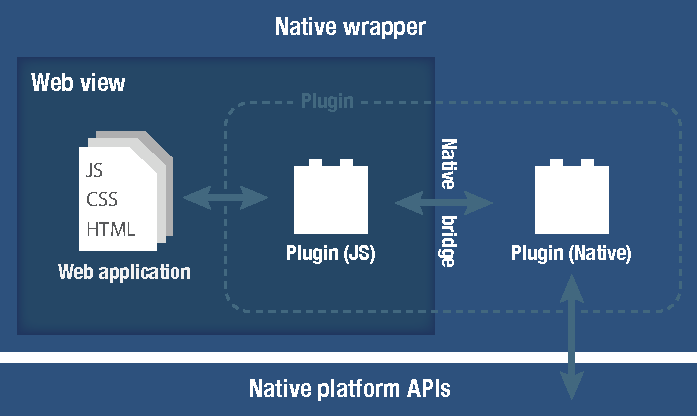
\includegraphics[width=\textwidth]{images/web-view-app-structure}
\caption{WebView app architecture: the application communicates with the native platform APIs via a plugin interface.\label{fig:web-view-app}}
\end{figure}

WebView apps wrap a web application in a native web view component, which in turn is hosted by a native wrapper (a native application). The web application can hook into the native APIs by means of plugins (referred to as modules by some frameworks). The plugins consist of a non-native part written in JavaScript and a native part implemented in one or more platform-specific languages. Data between these two parts is passed as serialized JSON via a native bridge, a JavaScript-to-native interface defined by the framework. Most of the inherent overhead in WebView apps is caused by the message passing through the native bridge as a result of data serialization/deserialization and the extra layers of abstraction. In this regard WebView app plugins share similar characteristics to that of application servers that query remote APIs for data. They both act as data providers that include a measurable query overhead (latency).

In addition to the inferior performance compared to native applications, one of the culprits of hybrid application development has been the lack of support for proper tooling --- a factor that lead companies such as Facebook and LinkedIn to pick native over HTML5 for their mobile applications \cite{html_vs_native_facebook}\cite{html_vs_native_linkedin} in 2012 and 2013, respectively. In the past, due to the lack of support for remote debugging, hybrid app developers had to resort to slow and brittle methods of littering code with print statements to debug their applications. This created a slow feedback loop that canceled out the productivity benefit of ``write once, run everywhere'' and made hybrid app development generally painful. It was not until 2011 when the first 3rd party hybrid app development tools, namely \textit{weinre} (WEb INspector REmote) and \textit{Apache Ripple}, emerged to address these issues. Powered by a feature-limited version of WebKit's (WK) Web Inspector, weinre allowed developers to remotely debug a web view like any other web application. Apache Ripple introduced a browser-based cross-platform emulator allowing developers to preview and debug their WebView apps and avoid slow deployments to an emulator or a device.

Support for hybrid app development tooling has seen significant improvement in the recent years. As browsers and mobile SDKs continue to mature, tools like weinre and Ripple are becoming legacy software. As of iOS 6.0 (released in late 2012) and Android 4.4 (released in late 2013) both iOS and Android smartphones ship with native support for remote debugging. As of this writing, weinre is still however the only viable option on some platforms (most notably, Windows Phone). Most of Ripple's core functionality has been superseded by newer browsers that have built-in support for various mobile device profiles and network simulation capabilities. Furthermore, emulators have become more efficient and are ever more suitable option for quick debugging. Ripple might still however prove itself useful in legacy setups that run outdated SDKs or older browser. Progress has also been made elsewhere in the industry as popular IDEs, such as Microsoft's Visual Studio and JetBrains' WebStorm, have recently integrated support for hybrid app development tools, and many hybrid mobile development platforms have developed new utilities to boost developer productivity. For example, hybrid app are nowadays able to sync and preview changes live on a device without a separate deployment using tools like \textit{PhoneGap Developer App} or \textit{Telerik AppBuilder Companion App}.

While the improved tooling has tackled many of the early challenges of developing WebView apps, the pitfalls of the underlying web view technology remain an issue. Even if web view performance is rarely an issue for less resource intensive WebView apps, developers still need to account for \textit{device fragmentation}. Device fragmentation is a real issue on Android, which as an open platform, allows vendors to introduce their own modifications to different versions of the software. Typically smarthpone vendors ship updates to the stock web view component on every major release. On Android however, as vendors are free to dictate which updates to apply, even phones running identical major versions are not guaranteed to have the exact same web view component. This causes issues for WebView app developers as the same target version might have different levels of support for certain web APIs and features.

Android addressed the fragmentation issue in its recent major release (Android 5.0) by decoupling the internal web view component into an \textit{updateable WebView}. This is good news for hybrid application development as phones running Android 5.0 or newer are now guaranteed to have an evergreen WebView that no longer depends on the OS update cycle. However, this implies that developers used to testing their applications against yearly major releases will now need to develop their WebView apps more like traditional web applications, in that their behaviour can potentially change (or break) at any time. To achieve a more consistent target to code to Android developers can leverage Intel's Crosswalk. Crosswalk is open-source runtime that bundles a modified version of Chromium (an open-source project behind the Google Chrome browser) with a given Android application to replace the stock WebView. It not only gives the developer a consistent web view (browser) to target, but also allows older Android phones (down until version 4.0) to benefit from the performance, security and feature updates of the newer Chromium. Hybrid development platforms like AppGyver Steroids, Ionic Platform and Intel XDK have already integrated support for Crosswalk.

have to remain concerned, however, is the increased size of the application caused by the bundled Chromium runtime.
- new chromium: crosswalk project / app size

new incarnation
- cross-platform native frameworks (xamarin, corona SDK, Appcelerator Titanium, react native, NativeScript)
	- tita, rn, ns: uses Javascript as the runtime to drive Native UI controls
	- uses a platform JS engine to talk to native APIs.

http://www.stevesouders.com/blog/2014/10/09/do-u-webview/
- new webviews (ios8, lollipop 5.0): wkvwebview (ios), chromium (android)
are brought almost on par with modern desktop browsers.
+ ease of development
+ platform support,
+ maintenance burden,IDEs, APIs
service worker, will-change property, push notifications
PhoneGap Build additionally includes Hydration, which checks for updates every time you open an app.
remain a very valid option for simple apps



\end{document}